\begin{exercise}
Consider the continuing MDP shown below.
The only decision to be made is that in the top state, where two actions are available, \textbf{left} and \textbf{right}.
The numbers show the rewards that are received deterministically after each action.
There are exactly two deterministic policies, $\pi_\textbf{left}$ and $\pi_\textbf{right}$.
What policy is optimal if $\gamma = 0$?
If $\gamma = 0.9$?
If $\gamma = 0.5$?

\begin{figure}[H]
    \centering
    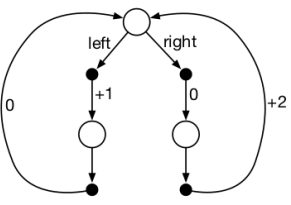
\includegraphics[width = 0.25 \textwidth]{2.20.png}
    \caption{}
    \label{fig:2.20}
\end{figure}

\end{exercise}

\begin{solution}
1. $\gamma = 0$: Since we discard all future rewards and only consider the immediate reward so we get

\begin{align*}
  v_{\pi_\textbf{right}}(\text{top}) = 0 \qquad
  v_{\pi_\textbf{left}}(\text{top}) = 1
\end{align*}

So in this case the optimal policy would be $\pi_\textbf{left}$.

2. $\gamma = 0.9$: With the Bellman equation \eqref{eq:2.14} we get

\begin{align*}
  v_{\pi_\textbf{right}}(\text{top})
  =
  0.9 \cdot v_{\pi_\textbf{right}}(\text{bottom})
  =
  0.9 \cdot (2 + 0.9 \cdot v_{\pi_\textbf{right}}(\text{top}))
  \implies
  v_{\pi_\textbf{right}}(\text{top}) = \frac{180}{19} \\
  v_{\pi_\textbf{left}}(\text{top})
  =
  1 + (0.9 \cdot v_{\pi_\textbf{left}}(\text{bottom}))
  =
  1 + 0.81 \cdot v_{\pi_\textbf{left}}(\text{top})
  \implies
  v_{\pi_\textbf{left}}(\text{top}) = \frac{100}{19}
\end{align*}

So in this case the optimal policy would be $\pi_\textbf{right}$.

3. $\gamma = 0.5$: With the Bellman equation \eqref{eq:2.14} we get:

\begin{align*}
v_{\pi_\textbf{right}}(\text{top})
=
0.5 \cdot v_{\pi_\textbf{right}}(\text{bottom})
=
0.5 \cdot (2 + 0.5 \cdot v_{\pi_\textbf{right}}(\text{top}))
\implies
v_{\pi_\textbf{right}}(\text{top}) = \frac{4}{3} \\
v_{\pi_\textbf{left}}(\text{top})
=
1 + (0.5 \cdot v_{\pi_\textbf{left}}(\text{bottom}))
=
1 + 0.25 \cdot v_{\pi_\textbf{left}}(\text{top})
\implies
v_{\pi_\textbf{left}}(\text{top}) = \frac{4}{3}
\end{align*}

So in this case both policies are optimal.
\end{solution}
